\documentclass[tikz,border=2pt]{standalone}
\usepackage{amsmath}
\usepackage{pgfplots}
\pgfplotsset{compat=1.18}

\begin{document}
% e is the base for which the exponential curve has slope exactly 1 at x=0 (tangent y=x+1);
% the sequence (1+1/n)^n climbs towards e ≈ 2.718.
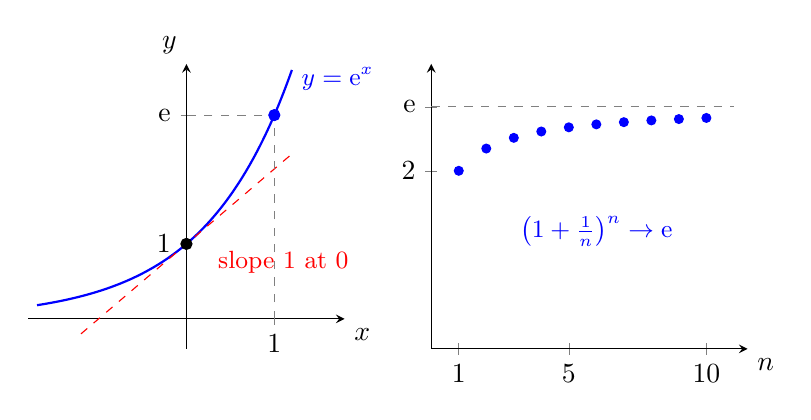
\begin{tikzpicture}
	\begin{axis}[
		name=left,
		axis lines=middle,
		xmin=-1.8, xmax=1.8,
		ymin=-0.4, ymax=3.4,
		xtick={1}, ytick={1,2.718}, yticklabels={$1$,$\mathrm{e}$},
		xlabel={$x$}, ylabel={$y$},
		xlabel style={below right}, ylabel style={above left},
		samples=120, smooth, clip=false,
		width=5.6cm, height=5.2cm
		]
		\addplot[thick, blue, domain=-1.7:1.2] {exp(x)};
		\addplot[red, dashed, domain=-1.2:1.2] {x+1};
		\addplot[only marks, mark=*, black] coordinates {(0,1)};
		\addplot[only marks, mark=*, blue] coordinates {(1,2.718)};
		\draw[dashed, gray] (axis cs:1,0) -- (axis cs:1,2.718) -- (axis cs:0,2.718);
		\node[blue, anchor=west, font=\small] at (axis cs:1.2,3.2) {$y=\mathrm{e}^x$};
		\node[red, anchor=west, font=\small] at (axis cs:0.25,0.75) {slope $1$ at $0$};
	\end{axis}
	\begin{axis}[
		at={(left.east)}, anchor=west, xshift=1.1cm,
		axis lines=middle,
		xmin=0, xmax=11.5,
		ymin=0, ymax=3.2,
		xtick={1,5,10}, ytick={2,2.718}, yticklabels={$2$,$\mathrm{e}$},
		xlabel={$n$}, ylabel={},
		xlabel style={below right},
		clip=false,
		width=5.6cm, height=5.2cm
		]
		\addplot[gray, dashed, domain=0:11] {2.71828};
		\addplot[only marks, mark=*, mark size=1.6pt, blue, samples at={1,...,10}] {(1+1/x)^x};
		\node[blue, anchor=north, font=\small] at (axis cs:6,1.6) {$\left(1+\tfrac1n\right)^n\to \mathrm{e}$};
	\end{axis}
\end{tikzpicture}
\end{document}
